\documentclass{beamer}

  \mode<presentation> {
    \usetheme{boxes}
    \usecolortheme{seagull}
  }
  
  \usepackage{pscyr}
  \usepackage[T2A]{fontenc}
  \usepackage[utf8]{inputenc}
  \usepackage[english, russian]{babel}
  \usepackage{graphicx}
  \usepackage{booktabs}
  \usepackage{amsmath,amsfonts,amssymb,amsthm,mathtools}
  \usepackage{euscript}
  \usepackage{mathrsfs} 

  %----------------------------------------------------------
  %   META
  %----------------------------------------------------------

  \title[ОТЧЕТ по производственной  практике]{Задача аппроксимации максимального стабильного моста в позиционной дифференциальной игре}  
  \author{Кощеев Никита}
  \institute[УрФУ]{Институт естественных наук и математики}
  \date{30 января 2018}

  \mathtoolsset{showonlyrefs=true}
  \graphicspath{ {images/} }


  \renewcommand{\rmdefault}{ftm}
  \newcommand{\dimension}{\mathbb{R}^2}


  %----------------------------------------------------------------------------------------
  %   TITLE PAGE
  %----------------------------------------------------------------------------------------
  
  \begin{document}
  
  \begin{frame}
      
    \titlepage 
    
  \end{frame}
  
  % \begin{frame}
  % \frametitle{Overview} 
  % \tableofcontents 
  % \end{frame}
  
  %----------------------------------------------------------------------------------------
  %   PRESENTATION SLIDES
  %----------------------------------------------------------------------------------------
  
  %------------------------------------------------
  \section{Постановка задачи} 
  %------------------------------------------------

  \begin{frame}
    \frametitle{Пример игры}
  
    \begin{equation}
        \frac{dx}{dt} = u + v, u \in P, v \in Q
    \end{equation}

    $R \subset \dimension$ - целевое множество 
    \vspace{5mm}
  
    $\theta$ - момент окончания игры

    Цель первого игрока: обеспечить $x(\theta) \in R$

    Цель второго игрока: обеспечить $x(\theta) \notin R$

  \end{frame}
  
  %------------------------------------------------
  
  \begin{frame}
    \frametitle{Стабильный мост}

    $W \in [t_0, \theta] \times \dimension$ - стабильный мост

    $W(\theta)=R$

    \begin{itemize}
      \item Применение оптимального управления первым игроком,
      при $x_0 \in W(t_0)$ гарантирует $x(\theta) \in R$
      \item Применение оптимального управления вторым игроком,
      при $x_0 \notin W(t_0)$ гарантирует $x(\theta) \notin R$
    \end{itemize}

  \end{frame}
  
  %------------------------------------------------
  
  \section{Решение}
  
  %------------------------------------------------
  
  \begin{frame}
    \frametitle{Алгоритм}

    $0=t_n, t_{n-1}, ..., t_1, t_0=\theta$

    $\Delta$ - шаг разбиения 

    Хотим получить набор \textit{t}-сечений моста W

    $S_i = W_i \oplus \Delta P$
    
    $W_{i+1} = S_i \ominus \Delta  Q$

  \end{frame}
  

  %------------------------------------------------
  
  \begin{frame}
    \frametitle{Алгебраическая сумма}
    
    Другое название - "сумма Минковского". 
    
    \begin{equation}
      A \oplus B =  \{ x + y | x \in A, y \in B \} 
    \end{equation}

    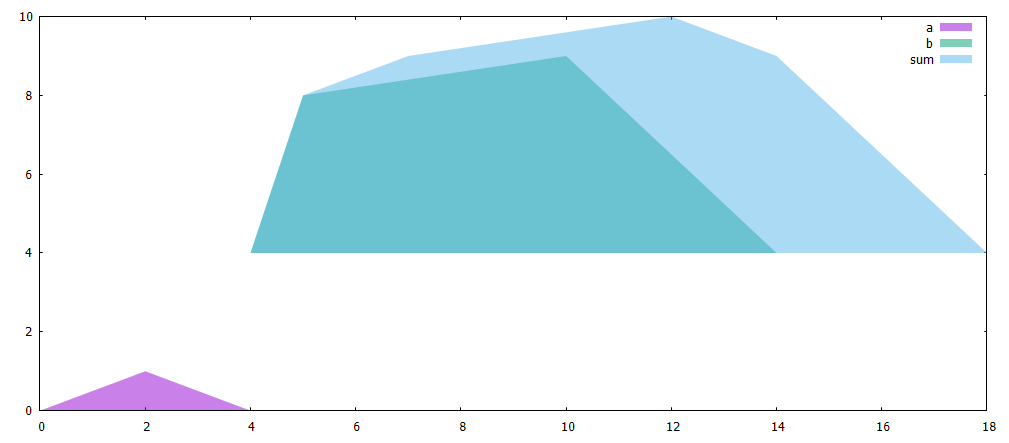
\includegraphics[width=1.0\textwidth]{minkowski_sum}
  
  \end{frame}
  
  %------------------------------------------------
  
  \begin{frame}
    \frametitle{Геометрическая разность}
    
    \begin{equation}
      A \ominus B =  \{ x | x + B \subseteq A \} 
    \end{equation}

    \begin{equation}
        A \ominus B =
        (\overline{\overline{A} \oplus (- B)})
    \end{equation}    

  \end{frame}
  
  %------------------------------------------------

  \subsection{CGAL} 
  
  \begin{frame}
    \frametitle{CGAL}
    
\includegraphics[width=1.0\textwidth]{cgal-logo}

    The Computational Geometry Algorithms Library

    Компоненты:

    \begin{itemize}
        \item 2D and 3D Linear Geometry Kernel
        \item 2D Polygons
        \item 2D Minkowski Sums
        \item 2D Polyline Simplification
    \end{itemize}

    \end{frame}

  %------------------------------------------------ 
  \begin{frame}
  \Huge{\centerline{Спасибо за внимание}}
  \end{frame}
  
  %----------------------------------------------------------------------------------------
  
  \end{document}